%%%%%%%%%%%%%%%%%%%%%%%%%%%%%%%%%%%%%%%%%
% Short Sectioned Assignment
% LaTeX Template
% Version 1.0 (5/5/12)
%
% This template has been downloaded from:
% http://www.LaTeXTemplates.com
%
% Original author:
% Frits Wenneker (http://www.howtotex.com)
%
% License:
% CC BY-NC-SA 3.0 (http://creativecommons.org/licenses/by-nc-sa/3.0/)
%
%%%%%%%%%%%%%%%%%%%%%%%%%%%%%%%%%%%%%%%%%

%----------------------------------------------------------------------------------------
%	PACKAGES AND OTHER DOCUMENT CONFIGURATIONS
%----------------------------------------------------------------------------------------

\documentclass[paper=a4, fontsize=11pt]{scrartcl} % A4 paper and 11pt font size

\usepackage{listings}
\usepackage{color}

\definecolor{dkgreen}{rgb}{0,0.6,0}
\definecolor{gray}{rgb}{0.5,0.5,0.5}
\definecolor{mauve}{rgb}{0.58,0,0.82}

\lstset{frame=tb,
language=Java,
aboveskip=3mm,
belowskip=3mm,
showstringspaces=false,
columns=flexible,
basicstyle={\small\ttfamily},
numbers=none,
numberstyle=\tiny\color{gray},
keywordstyle=\color{blue},
commentstyle=\color{dkgreen},
stringstyle=\color{mauve},
breaklines=true,
breakatwhitespace=true,
tabsize=3
}

\usepackage[T1]{fontenc} % Use 8-bit encoding that has 256 glyphs
\usepackage[utf8]{inputenc}
\usepackage[spanish]{babel} % English language/hyphenation
\usepackage{amsmath,amsfonts,amsthm} % Math packages
% \usepackage{breakcites}
\usepackage{sectsty} % Allows customizing section commands
\allsectionsfont{\centering \normalfont\scshape} % Make all sections centered, the default font and small caps
\usepackage{algorithm}
\usepackage{url}
\usepackage[noend]{algpseudocode}
\makeatletter
\usepackage{graphicx}

\usepackage{fancyhdr} % Custom headers and footers
\pagestyle{fancyplain} % Makes all pages in the document conform to the custom headers and footers
\fancyhead{} % No page header - if you want one, create it in the same way as the footers below
\fancyfoot[L]{} % Empty left footer
\fancyfoot[C]{} % Empty center footer
\fancyfoot[R]{\thepage} % Page numbering for right footer
\renewcommand{\headrulewidth}{0pt} % Remove header underlines
\renewcommand{\footrulewidth}{0pt} % Remove footer underlines
\setlength{\headheight}{13.6pt} % Customize the height of the header
% Reinsert missing \algbackskip
\def\algbackskip{\hskip-\ALG@thistlm}
\renewcommand*{\ALG@name}{Algoritmo}
% \makeatother
\decimalpoint
\numberwithin{equation}{section} % Number equations within sections (i.e. 1.1, 1.2, 2.1, 2.2 instead of 1, 2, 3, 4)
\numberwithin{figure}{section} % Number figures within sections (i.e. 1.1, 1.2, 2.1, 2.2 instead of 1, 2, 3, 4)
\numberwithin{table}{section} % Number tables within sections (i.e. 1.1, 1.2, 2.1, 2.2 instead of 1, 2, 3, 4)

\setlength\parindent{0pt} % Removes all indentation from paragraphs - comment this line for an assignment with lots of text

%----------------------------------------------------------------------------------------
%	TITLE SECTION
%----------------------------------------------------------------------------------------

\newcommand{\horrule}[1]{\rule{\linewidth}{#1}} % Create horizontal rule command with 1 argument of height

\title{	
\normalfont \normalsize 
\textsc{Universidad Nacional de San Agustín, Escuela de Ingenieria de Sistemas} \\ [25pt] % Your university, school and/or department name(s)
\horrule{0.5pt} \\[0.4cm] % Thin top horizontal rule
\huge ADA - Lab 05 \\ % The assignment title
\horrule{2pt} \\[0.5cm] % Thick bottom horizontal rule
}

\author{Fernando Enrique Araoz Morales - 20173373} % Your name

\date{\normalsize\today} % Today's date or a custom date

\begin{document}

\maketitle % Print the title

%----------------------------------------------------------------------------------------
%	PROBLEM 1
%----------------------------------------------------------------------------------------

\section{Introducción}\label{sec:introducción}

En este documento se presenta la implementación de la estructura Heap, MinHeap, MaxHeap, así como
la comparación del tiempo de ejecución de este algoritmo contra Merge sort y Quick sort usando
diferentes elementos (aleatorio, ordenado, inverso, únicos).


\section{Heap}\label{sec:heap}

    La estructura Heap es una estructura sencilla de implementar.
    Consta de un array de elementos, un método siftDown que se encarga de tomar el elemento raiz
    y reubicarlo en su posicion adecuada, un método heapify que se encarga de crear el Heap a partir
    de un array cualquiera, y un método sort que usa estos métodos para ordenar el array 'in-place'.


    El código en sí se encuentra organizado de la siguiente manera:
    Una clase abstracta BinaryHeap<T>, esta representa un Heap cualquiera, y contiene toda la
    implementación necesaria, excepto un método compare().
    Este método es el que define si es un Max o Min heap, por lo tanto las clases que lo hereden
    son responsables de implementarlo.

    Las clases MaxBinaryHeap y MinBinaryHeap simplemente heredan de la clase BinaryHeap e implementan
    el método compare() según sea adecuado.

\begin{lstlisting}



public abstract class BinaryHeap<T extends Comparable<T>> {

    private final T[] arr;

    public BinaryHeap(T[] arr) {
        this.arr = arr;
    }

    private void swap(int pos1, int pos2) {
        T buffer = arr[pos1];
        arr[pos1] = arr[pos2];
        arr[pos2] = buffer;
    }

    void heapify() {

        int lastPos = arr.length;
        int firstParent = (lastPos % 2 == 0)? (lastPos - 2) / 2: (lastPos - 1) / 2;

        for (int i = firstParent; i >= 0; i--) {
            siftDown(i, arr.length);
        }

    }

    abstract boolean compare(T a, T b);

    private void siftDown(int pos, int maxPos) {
        int largestPos = pos;
        int posLeft = pos * 2 + 1;
        int posRight = pos * 2 + 2;

        if (posLeft < maxPos && compare(arr[posLeft], arr[largestPos])) {
            largestPos = posLeft;
        }

        if (posRight < maxPos && compare(arr[posRight], arr[largestPos])) {
            largestPos = posRight;
        }


        if (largestPos != pos) {
            swap(pos, largestPos);

            siftDown(largestPos, maxPos);
        }

    }

    void sort() {
        this.heapify();
        for (int max = arr.length; max > 0; --max) {
            swap(0, max - 1);
            this.siftDown(0, max - 1);
        }
    }

    @Override
    public String toString() {
        StringBuilder res = new StringBuilder("[");
        for (T i: arr) {
            res.append(i).append(", ");
        }
        res.append("]");

        return res.toString();
    }

}


\end{lstlisting}



% \begin{figure}
%     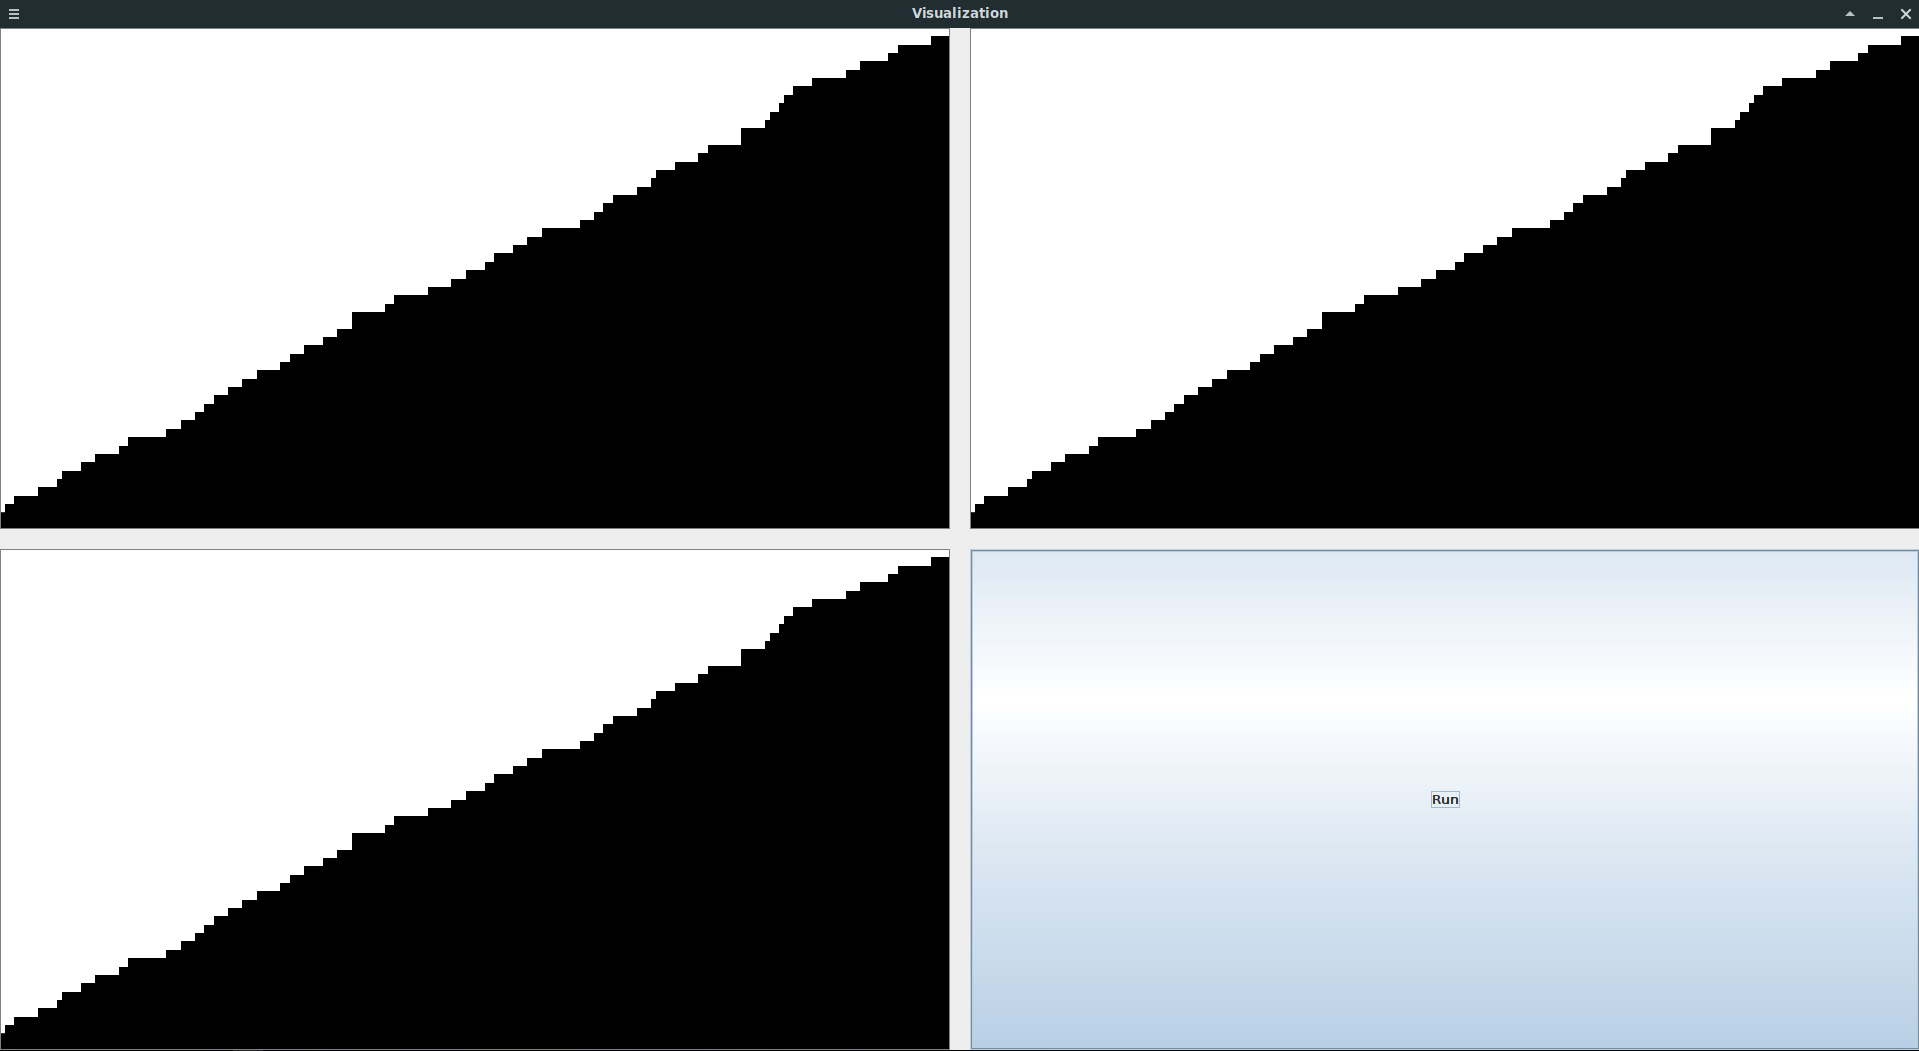
\includegraphics[width=\linewidth]{Resultado.png}
%     \caption{Resultado.}
% \end{figure}


%------------------------------------------------

\end{document}
